% Шрифт всего документа - 12pt. Тип документа - статья
\documentclass[12pt]{article}

% Параметры документа (дисциплина, тема, преподаватель и т.п.)
% Загружаем первым, чтобы флаги из config.tex были доступны в преамбуле
% ==========================================
% ШРИФТЫ
% ==========================================

% Шрифт выбирается автоматически под ОС
\usepackage{ifplatform}

\iflinux
    \newcommand{\mainfont}{Liberation Serif}
    \newcommand{\monofont}{Liberation Mono}
    \newcommand{\monofontcyr}{Liberation Mono}
\else
    \newcommand{\mainfont}{Times New Roman}
    \newcommand{\monofont}{Courier New}
    \newcommand{\monofontcyr}{Menlo}
\fi

% ==========================================
% ПАРАМЕТРЫ ДОКУМЕНТА
% ==========================================

% Библиография:
\newif\ifbib \bibtrue

% Графики функций (pgfplots):
\newif\ifplots \plotsfalse

% Схемы и диаграммы (tikz):
\newif\iftikz \tikzfalse

% Листинг кода (minted):
\newif\iflisting \listingtrue

% Кафедра (две строки)
\newcommand{\kafedraFirstString}{прикладной}
\newcommand{\kafedraSecondString}{математики}

% Дисциплина
\newcommand{\discipline}{Теория функций комплексного переменного и дифференциальные уравнения в частных производных}

% Данные студента
\newcommand{\courseYear}{3}
\newcommand{\levelEducation}{бакалавриата}
\newcommand{\group}{ИДБ-23-14}
\newcommand{\lastName}{Дамакальщиков}
\newcommand{\firstName}{М.}
\newcommand{\middleName}{А.}

% Тема работы
\newcommand{\topic}{Уравнение конвекции--реакции--диффузии для примеси}

% Направление и профиль подготовки
\newcommand{\specialization}{09.03.03 Прикладная информатика}
\newcommand{\trainingProfile}{Математическое и компьютерное моделирование процессов и систем}

% Руководитель курсовой работы (Ф.И.О., должность, степень, звание)
\newcommand{\supervisor}{ст. преп. Девятерикова Е. А.}

% Год в колонтитуле
\newcommand{\yearFooter}{2026}

% ==========================================
% СОБСТВЕННЫЕ КОМАНДЫ
% ==========================================

% Секция без нумерации
\newcommand{\unnsection}[1]{
    \clearpage
    \section*{#1}
    \addcontentsline{toc}{section}{#1}
    % Обновляем колонтитул вручную: \section* не вызывает \markboth
    \markboth{#1}{#1}
    % На странице с заголовком раздела убираем верхний колонтитул и черту,
    % чтобы не дублировать название раздела (оно уже есть в виде H1)
    \thispagestyle{plain}
}

% Подсекция без нумерации
\newcommand{\unnsubsection}[1]{
    \subsection*{#1}
    \addcontentsline{toc}{subsection}{#1}
}

% Подподсекция без нумерации
\newcommand{\unnsubsubsection}[1]{
    \subsubsection*{#1}
    \addcontentsline{toc}{subsubsection}{#1}
}


% ==========================================
% ШРИФТЫ И ЯЗЫКИ
% ==========================================

% Управление шрифтами
\usepackage{fontspec}
% Основной шрифт документа (задаётся в config.tex)
\setmainfont{\mainfont}

% Моноширинный шрифт (для листингов кода, задаётся в config.tex)
\setmonofont{\monofont}

% Поддержка многоязычных документов (русский + английский + немецкий + французский)
\usepackage{polyglossia}
\setdefaultlanguage{russian}
\setotherlanguage[variant=german]{german}
\setotherlanguage{english}
\setotherlanguage{french}

% Кириллический моноширинный шрифт (задаётся в config.tex)
\newfontfamily\cyrillicfonttt{\monofontcyr}

% ==========================================
% МАТЕМАТИКА
% ==========================================

% Расширенные математические формулы и окружения
\usepackage{amsmath}

% Дополнительные математические символы (\mathbb и др.)
\usepackage{amssymb}

% Запятая как разделитель дробной части (вместо точки)
\usepackage{icomma}

% ==========================================
% ТАБЛИЦЫ
% ==========================================

% Расширенные типы столбцов (m{}, b{}, >{}, <{} и др.)
\usepackage{array}

% Профессиональное оформление линий (\toprule, \midrule, \bottomrule)
\usepackage{booktabs}

% ==========================================
% ГРАФИКА И ЦВЕТА
% ==========================================

% Вставка и масштабирование изображений
\usepackage{graphicx}
% Путь к изображениям
\graphicspath{{./images/}}

% Подрисунки (несколько изображений в одном окружении figure)
\usepackage{subcaption}

% Обтекание изображений текстом
\usepackage{wrapfig}

% Выравнивание по центру подписей под портретами
\captionsetup[wrapfigure]{justification=centering, singlelinecheck=false}

% Точное позиционирование плавающих объектов (спецификатор H)
\usepackage{float}

% Поддержка цветов
\usepackage{xcolor}

% ==========================================
% НАСТРОЙКА СТРАНИЦЫ
% ==========================================

% Настройка полей документа
\usepackage[a4paper, margin=2cm]{geometry}

% Настройка ориентаций страниц
\usepackage{pdflscape}

% Кастомизация колонтитулов
\usepackage{fancyhdr}
\setlength{\headheight}{15pt}

% Основной стиль страниц: название раздела сверху курсивом, горизонтальная черта под ним и номер страницы внизу по центру
\fancypagestyle{main}{
    \fancyhf{}                                              % очистить все поля
    \fancyhead[L]{\textit{\nouppercase{\leftmark}}}         % раздел в шапке
    \fancyfoot[C]{\thepage}                                 % номер страницы
    \renewcommand{\headrulewidth}{0.6pt}                    % линия под шапкой
    \renewcommand{\footrulewidth}{0pt}                      % без линии в футере
}

% Стиль страницы, на которой начинается новый раздел: шапки и черты нет
\fancypagestyle{plain}{
    \fancyhf{}
    \fancyfoot[C]{\thepage}
    \renewcommand{\headrulewidth}{0pt}
    \renewcommand{\footrulewidth}{0pt}
}

% ==========================================
% PDF И ССЫЛКИ
% ==========================================

% Кликабельные ссылки в PDF
\usepackage[colorlinks=true, urlcolor=blue, linkcolor=black, citecolor=black]{hyperref}

% Улучшенное управление закладками PDF
\usepackage{bookmark}

% ==========================================
% СОДЕРЖАНИЕ
% ==========================================

% Настройка отображения содержания (точки между заголовком и номером страницы)
\usepackage{tocloft}
\renewcommand{\cftdot}{.}
\renewcommand{\cftsecdotsep}{\cftdotsep}

% ==========================================
% ОПЦИОНАЛЬНЫЕ ПАКЕТЫ
% Управляются флагами в config.tex
% ==========================================

% Библиография в стиле ГОСТ (флаг \bibtrue)
\ifbib
    \usepackage[backend=biber, style=gost-numeric, language=autobib, autolang=other]{biblatex}
    \addbibresource{references.bib}
\fi

% Графики функций (флаг \plotstrue)
\ifplots
    \usepackage{pgfplots}
    \pgfplotsset{compat=1.18}
    \pgfplotsset{/pgf/number format/use comma}
\fi

% Схемы и диаграммы (флаг \tikztrue)
\iftikz
    \usepackage{tikz}
    \usetikzlibrary{shapes.geometric, arrows.meta, positioning, calc}
\fi

% Листинги кода с подсветкой синтаксиса (флаг \listingtrue)
\iflisting
    \usepackage{minted}
    \setminted{
        fontsize=\small,
        linenos=true,
        breaklines=true,
        frame=single
    }
\fi

% Начало документа
\begin{document}

    % Отключает нумерацию страниц в титульном листе и в содержании
    \pagenumbering{gobble}

    % Титульная страница
    % Титульная страница
\begin{titlepage}

    % Логотип вуза
    \begin{figure}
        \centering
        
\includegraphics[width=0.35\linewidth]{logo.png}
    \end{figure}

    % Подпись под логотипом
    \begin{center}
        \textbf{МИНОБРНАУКИ РОССИИ} \\[2pt]
        \textbf{Федеральное государственное автономное образовательное учреждение} \\
        \textbf{высшего образования} \\
        \textbf{<<Московский государственный технологический университет <<СТАНКИН>>} \\
        \textbf{(ФГАОУ ВО <<МГТУ <<СТАНКИН>>)} \\[4pt]
        % Разделительная линия
        \hrule
    \end{center}

    % Институт
    \noindent
    \begin{minipage}[t]{0.5\textwidth}
        \raggedright
        \textbf{Институт} \\
        \textbf{информационных} \\
        \textbf{технологий}
    \end{minipage}
    % Кафедра
    \hfill
    \begin{minipage}[t]{0.5\textwidth}
        \raggedleft
        \textbf{Кафедра} \\
        \textbf{\kafedraFirstString} \\
        \textbf{\kafedraSecondString}
    \end{minipage}
    \vspace{1.5cm}

    % Название и тип работы
    \begin{center}
        {\large\textbf{КУРСОВАЯ РАБОТА}} \\[6pt]
        По дисциплине: \\[4pt]
        \parbox{0.65\textwidth}{\centering <<\discipline>>}
    \end{center}
    \vspace{0.5cm}

    % Тема работы
    \begin{center}
        На тему: \\[4pt]
        <<\topic>>
    \end{center}
    \vspace{1.5cm}

    % Направление и профиль подготовки
    \noindent
    \begin{minipage}[t]{0.5\textwidth}
        \raggedright
        Направление подготовки: \\[5pt]
        Профиль:
    \end{minipage}
    \begin{minipage}[t]{0.5\textwidth}
        \raggedleft
        \specialization \\[5pt]
        \trainingProfile
    \end{minipage}
    \vspace{1cm}

    % Выполнил
    \noindent
    \begin{minipage}[t]{0.2\textwidth}
        \raggedright
        Выполнил:
    \end{minipage}
    \begin{minipage}[t]{0.55\textwidth}
        \centering
        \underline{\makebox[8cm]{ИДБ-23-14 \lastName~\firstName~\middleName}} \\
        {\small\textit{(группа, Ф.И.О.)}}
    \end{minipage}
    \hfill
    \begin{minipage}[t]{0.18\textwidth}
        \centering
        \underline{\makebox[2.5cm]{\vphantom{\lastName}}} \\
        {\small\textit{(подпись)}}
    \end{minipage}
    \vspace{0.8cm}

    % Руководитель
    \noindent
    \begin{minipage}[t]{0.2\textwidth}
        \raggedright
        Руководитель:
    \end{minipage}
    \begin{minipage}[t]{0.55\textwidth}
        \centering
        \underline{\makebox[8cm]{\supervisor}} \\
        {\small\textit{(Ф.И.О., должность, степень, звание)}}
    \end{minipage}
    \hfill
    \begin{minipage}[t]{0.18\textwidth}
        \centering
        \underline{\makebox[2.5cm]{\vphantom{\supervisor}}} \\
        {\small\textit{(подпись)}}
    \end{minipage}
    \vspace{1cm}

    % Оценка
    \noindent
    Оценка:~~~\underline{\makebox[3cm]{\vphantom{\supervisor}}}

    \vfil

    % Колонтитул
    \enlargethispage{3cm}
    \centering
    \small Москва, \yearFooter~г.

\end{titlepage}


    % Содержание (без верхнего колонтитула и номера страницы)
    \begin{center}
        \tableofcontents
    \end{center}
    \thispagestyle{empty}

    % Новая страница
    \newpage

    % Нумерация с 3-его номера
    \pagenumbering{arabic}
    \setcounter{page}{3}

    % Включаем кастомный стиль колонтитулов для содержания
    \pagestyle{main}

    % ==========================================
    % СОДЕРЖАНИЕ ОТЧЁТА
    % ==========================================

    \unnsection{Историческая справка}

    Уравнение конвекции--реакции--диффузии --- это параболическое дифференциальное
    уравнение в частных производных, которое описывает эволюцию концентрации некоторого
    вещества \textit{(примеси, химического реагента, биологической популяции)} под действием
    трёх одновременно протекающих процессов: молекулярной диффузии, конвективного переноса
    с потоком среды и локального источника или стока, обусловленного химической реакцией.

    Историческая особенность данного уравнения состоит в том, что каждый из трёх его
    механизмов имеет собственную, относительно независимую историю и сформировался в рамках
    своей научной традиции --- теории теплопроводности и молекулярной диффузии \textit{(XIX век)},
    химической кинетике \textit{(вторая половина XIX -- начало XX века)} и гидродинамики сплошных
    сред \textit{(с XVIII века)}.

    Объединение этих трёх линий в одно уравнение произошло лишь в первой половине XX века:
    сначала в работе Колмогорова, Петровского и Пискунова 1937 года, где впервые строго
    рассматривалось уравнение, объединяющие диффузию с нелинейной реакцией, а затем в работах
    советской школы теории горения \textit{(Зельдович Я. Б., Франк-Каменецкий Д. А.)}, где
    появилась полная триада <<конвекция--диффузия--реакция>>.

    Дальнейшее изложение организовано в соответствии с этой логикой: сначала рассматривается
    каждая из трёх линий по отдельности, затем --- их объединение, и в заключение --- современные постановки задач.


% =====================================================================
\unnsubsection{Зарождение теории диффузии}
% ---------------------------------------------------------------------
% Объём: ~1 страница.
%
% Ключевые имена и даты:
%   - Жозеф Фурье (1822) — теплопроводность как математическая основа.
%   - Томас Грэм (1828–1833) — первые количественные эксперименты
%     с диффузией газов.
%   - Адольф Фик (1855) — первый и второй законы диффузии по аналогии
%     с законом Фурье; рождение уравнения диффузии.
%   - Роберт Браун (1827) — наблюдение броуновского движения.
%   - Альберт Эйнштейн (1905) — статистическая теория.
%   - Мариан Смолуховский (1906) — независимый вывод.
%   - Жан Перрен (1909, Нобелевская премия 1926) —
%     экспериментальная проверка.
%
% Формулы для включения:
%   - Первый закон Фика: j = -D · ∂c/∂x  (аналогия с Фурье и Омом).
%   - Второй закон Фика (вывод из закона сохранения вещества).
%   - Соотношение Эйнштейна-Смолуховского: <R^2> = 6 D t.
%
% Источники: Mehrer & Stolwijk (разделы 2.1, 2.2, 2.5);
%            оригинальная статья Фика (1855);
%            Wikipedia «Diffusion equation».
% =====================================================================

% TODO: подраздел


% =====================================================================
\unnsubsection{Химическая кинетика и реакционное слагаемое}
% ---------------------------------------------------------------------
% Объём: ~0,5–1 страница.
%
% Ключевые имена и даты:
%   - К. Гульдберг и П. Вааге (1864) — закон действующих масс.
%   - Сванте Аррениус (1889) — температурная зависимость скорости
%     реакции.
%   - Н.Н. Семёнов (Нобелевская премия по химии 1956) — теория
%     цепных реакций; основание советской школы химической кинетики
%     и теории горения.
%   - Д.А. Франк-Каменецкий — мост от химической кинетики к теории
%     горения и к уравнению конвекции-реакции-диффузии.
%
% Формулы для включения:
%   - Закон Аррениуса: k = k_0 · exp(-E / RT).
%   - Краткое пояснение, почему именно эта зависимость делает
%     уравнение конвекции-реакции-диффузии существенно нелинейным.
%
% Источники: Wikipedia «Закон действующих масс»;
%            Mehrer & Stolwijk (раздел 2.4);
%            предисловие к Зельдовичу и др.
% =====================================================================

% TODO: подраздел


% =====================================================================
\unnsubsection{Уравнение Колмогорова--Петровского--Пискунова}
% ---------------------------------------------------------------------
% Объём: ~1–1,5 страницы. Это исторический центр раздела.
%
% Ключевые имена и даты:
%   - А.Н. Колмогоров, И.Г. Петровский, Н.С. Пискунов (1937) —
%     уравнение КПП в контексте биологической задачи о распространении
%     доминантного гена в популяции.
%   - Р.А. Фишер (1937) — параллельная независимая работа о волне
%     преимущественного гена.
%   - Современное название: уравнение Фишера-КПП.
%
% Формулы для включения (из оригинальной статьи КПП-1937):
%   - Исходное уравнение:
%       ∂v/∂t = k · ∂^2 v/∂x^2 + F(v),
%       при F(0) = F(1) = 0,   F(v) > 0 на (0, 1),
%       F'(0) = α > 0,         F'(v) < α на (0, 1).
%   - Скорость предельной бегущей волны:  λ_0 = 2 √(k α).
%   - Уравнение для предельной формы кривой плотности:
%       λ_0 · dv/dx = k · d^2 v/dx^2 + F(v).
%
% Источники: оригинал КПП-1937 (КПП-1937.pdf в папке источников);
%            Wikipedia «Fisher's equation».
% =====================================================================

% TODO: подраздел


% =====================================================================
\unnsubsection{Рождение полного уравнения}
% ---------------------------------------------------------------------
% Объём: ~1 страница. Кульминация раздела — момент, когда «триада»
% (конвекция + диффузия + реакция) собирается воедино в осмысленной
% физической задаче.
%
% Ключевые имена и даты:
%   - Я.Б. Зельдович и Д.А. Франк-Каменецкий (1930–40-е) — теория
%     ламинарного пламени; уравнения распространения пламени, в которых
%     впервые присутствуют все три слагаемых.
%   - Л.Д. Ландау и G. Darrieus — гидродинамическая неустойчивость
%     плоского фронта пламени.
%   - Гидродинамическая основа конвективного слагаемого:
%     Эйлер, Навье-Стокс (упомянуть кратко).
%
% Формулы для включения (из §4 главы 1 монографии Зельдовича и др.):
%   ρ u c · dT/dx = d/dx(λ · dT/dx) + Q · W(a, T)
%   ρ u   · da/dx = d/dx(ρ D · da/dx) − W(a, T)
%
% Здесь явно видны:
%   - конвективные слагаемые ρ u c · d/dx и ρ u · d/dx;
%   - диффузионные слагаемые d/dx(λ · d/dx) и d/dx(ρ D · d/dx);
%   - реакционные слагаемые Q · W и W со скоростью реакции W(a, T),
%     содержащей закон Аррениуса.
%
% При желании — формула нормальной скорости пламени u_n.
%
% Источники: Зельдович и др. (предисловие; глава 1, §4).
% =====================================================================

% TODO: подраздел


% =====================================================================
\unnsubsection{Современные постановки и области применения}
% ---------------------------------------------------------------------
% Объём: ~0,5–1 страница. Плавный переход к разделу
% «Постановка задачи».
%
% Направления применения:
%   - Перенос примеси в атмосфере и водоёмах (школа Г.И. Марчука) —
%     прямая связь с темой курсовой.
%   - Полупроводниковая физика: drift-diffusion equation для
%     концентраций электронов и дырок.
%   - Реакционно-диффузионные системы в биологии: А. Тьюринг (1952) —
%     морфогенез, образование пятен и полос.
%   - Гидрогеология, химические реакторы, теплоперенос в твёрдых телах.
%
% Источники: Wikipedia «Convection-diffusion equation»;
%            Г.И. Марчук «Математическое моделирование в проблеме
%            окружающей среды».
% =====================================================================

% TODO: подраздел

    \unnsection{Постановка задачи}

    В исторической справке было показано, как уравнение конвекции--реакции--диффузии
    сложилось в единый математический объект, объединивший молекулярную диффузию,
    конвективный перенос и химическую реакцию. В настоящем разделе это уравнение
    формулируется как корректная краевая задача, после чего обзорно рассматриваются
    основные подходы к её решению. Раздел носит \textit{обзорный} характер: его цель ---
    систематизировать способы решения уравнения и указать границы их применимости,
    а не довести до конца вывод какого-либо одного из них.

    \unnsubsection{Математическая постановка краевой задачи}

        Пусть $\Omega \subset \mathbb{R}^n$~--- пространственная область с границей $\partial\Omega$,
        а $(0, T]$~--- рассматриваемый промежуток времени.
        Искомая величина~--- концентрация примеси $c(\mathbf{x}, t)$,
        удовлетворяющая в области $\Omega \times (0, T]$ уравнению
        \[
            \frac{\partial c}{\partial t}
            + \mathbf{u} \cdot \nabla c
            = \nabla \cdot (D\,\nabla c)
            + R(c),
        \]
        где $\mathbf{u}(\mathbf{x}, t)$~--- поле скоростей среды \textit{(конвективный перенос)},
        $D$~--- коэффициент диффузии \textit{(в общем случае тензор)},
        а $R(c)$~--- реакционный член.

        Для однозначной разрешимости уравнение дополняется \textit{начальным условием}
        \[
            c(\mathbf{x}, 0) = c_0(\mathbf{x}), \qquad \mathbf{x} \in \Omega,
        \]
        и \textit{граничными условиями} на $\partial\Omega$, которые традиционно
        разделяют на три типа. Условие \textit{первого рода} \textit{(Дирихле)} задаёт
        концентрацию на границе, $c\big|_{\partial\Omega} = g$; условие \textit{второго рода}
        \textit{(Неймана)} задаёт диффузионный поток,
        $-D\,\dfrac{\partial c}{\partial n}\big|_{\partial\Omega} = q$
        \textit{(в частности, $q = 0$ отвечает непроницаемой стенке)};
        условие \textit{третьего рода} \textit{(Робена)} описывает массообмен
        с окружением, $-D\,\dfrac{\partial c}{\partial n}\big|_{\partial\Omega}
        = \beta\,(c - c_\infty)$.
        Совокупность <<уравнение~$+$~начальное условие~$+$~граничные условия>>
        образует корректно поставленную \textit{(по Адамару)} краевую задачу.

        Для аналитического изучения и для примера расчёта удобна одномерная
        каноническая форма уравнения с постоянными коэффициентами:
        \[
            \frac{\partial c}{\partial t}
            + v\,\frac{\partial c}{\partial x}
            = D\,\frac{\partial^2 c}{\partial x^2}
            + R(c),
            \qquad x \in (0, L), \quad t > 0.
        \]

        Характер задачи и выбор метода решения во многом определяются двумя
        безразмерными параметрами:
        \[
            \mathrm{Pe} = \frac{v L}{D}, \qquad
            \mathrm{Da} = \frac{\tau_{\mathrm{conv}}}{\tau_{\mathrm{reac}}}.
        \]
        Число Пекле $\mathrm{Pe}$ выражает соотношение конвективного и диффузионного
        переноса: при $\mathrm{Pe} \ll 1$ преобладает диффузия и уравнение близко к
        классическому уравнению теплопроводности, а при $\mathrm{Pe} \gg 1$ преобладает
        конвекция и уравнение приобретает почти гиперболический, транспортный характер.
        Число Дамкёлера $\mathrm{Da}$ выражает отношение характерного времени переноса
        к характерному времени реакции, то есть относительную интенсивность
        реакционного слагаемого.

    \unnsubsection{Аналитические методы}

        Решение в замкнутой форме удаётся получить лишь для узкого класса задач:
        линейный \textit{(или отсутствующий)} реакционный член, постоянные коэффициенты,
        простая геометрия области.

        \textbf{Линейное уравнение с постоянными коэффициентами.}
        Для \textit{чистой диффузии} ($v = 0$, $R = 0$) в ограниченной области применяется
        метод разделения переменных \textit{(метод Фурье)}, а в неограниченной --- фундаментальное
        решение в виде ядра теплопроводности. Уравнение \textit{конвекции--диффузии}
        с постоянной скоростью $v$ переходом в подвижную систему координат
        $\xi = x - v t$ сводится к чисто диффузионному; его фундаментальное решение ---
        сносимый потоком гауссов профиль
        \[
            c(x, t) = \frac{1}{\sqrt{4\pi D t}}\,
            \exp\!\left(-\frac{(x - v t)^2}{4 D t}\right).
        \]
        \textit{Линейная реакция} первого порядка $R = -k c$ устраняется подстановкой
        $c = e^{-k t}\,w(x, t)$, после чего задача снова сводится к конвекции--диффузии.
        Общие линейные задачи решаются интегральными преобразованиями
        \textit{(Фурье, Лапласа)} и методом функций Грина~\cite{tihonovSamarskii1999}.

        \textbf{Нелинейная реакция.}
        Ключевой приём здесь~--- поиск решения в виде \textit{бегущей волны}
        $c(x, t) = \varphi(x - \lambda t)$: такая подстановка превращает уравнение
        в частных производных в обыкновенное дифференциальное уравнение для профиля
        $\varphi(\xi)$. Именно так получаются фронты Колмогорова--Петровского--Пискунова---Фишера
        с минимальной скоростью $\lambda_0 = 2\sqrt{D\,\alpha}$, встречавшиеся в
        исторической справке~\cite{kpp1937}, и фронты горения
        Зельдовича--Франк-Каменецкого~\cite{zeldovich1944}. Бегущая волна и есть
        математический образ фронта пламени. Помимо неё используются автомодельные
        \textit{(self-similar)} решения, опирающиеся на инвариантность задачи
        относительно растяжений, а для уравнений с нелинейной конвекцией
        \textit{(типа уравнения Бюргерса)}~--- линеаризующее преобразование Коула--Хопфа.

        Аналитические методы дают точные, физически прозрачные результаты, однако
        охватывают лишь идеализированные постановки. В большинстве практических задач
        приходится прибегать к численному решению.

    \unnsubsection{Численные методы}

        При переменном поле скоростей, нелинейном реакционном члене, сложной геометрии
        области или нескольких пространственных измерениях замкнутого решения не существует,
        и уравнение решается приближённо.

        \textbf{Метод конечных разностей.}
        Область покрывается сеткой по пространству и времени, а производные заменяются
        разностными отношениями. \textit{Явные} схемы \textit{(прямой метод Эйлера)} просты
        в реализации, но условно устойчивы~--- шаг по времени ограничен условием типа
        Куранта. \textit{Неявные} схемы \textit{(обратный метод Эйлера, схема Кранка--Николсон)}
        безусловно устойчивы ценой решения системы линейных алгебраических уравнений
        на каждом шаге. Особую трудность создаёт конвективное слагаемое при больших
        числах Пекле: центральные разности порождают нефизичные осцилляции решения,
        поэтому применяют противопотоковые \textit{(upwind)} схемы и схемы с искусственной
        вязкостью~\cite{samarskii1977}.

        \textbf{Метод прямых.}
        Дискретизация только по пространству превращает уравнение в частных производных
        в систему обыкновенных дифференциальных уравнений по времени, которую решают
        стандартными интеграторами для жёстких систем.

        \textbf{Методы расщепления.}
        Поскольку оператор уравнения естественно распадается на три качественно различные
        части~--- конвекцию, диффузию и реакцию,~--- их удобно учитывать поочерёдно,
        решая каждую подзадачу наиболее подходящим для неё методом
        \textit{(расщепление Марчука--Стрэнга)}~\cite{marchukSplitting1988}. Этот приём
        особенно органичен именно для уравнения конвекции--реакции--диффузии.

        \textbf{Методы конечных элементов и конечных объёмов.}
        Метод конечных элементов удобен для областей сложной геометрии, а метод конечных
        объёмов обеспечивает точное выполнение закона сохранения вещества, что важно
        для задач переноса.

    \unnsubsection{Феноменологические и экспериментально-статистические подходы}

        В наиболее сложных режимах фронт реакции теряет устойчивость и фрагментируется
        \textit{(интенсивная реакция, неустойчивости Дарье--Ландау и диффузионно-тепловая
        неустойчивость при малых числах Льюиса)}. Решение задачи становится сложной,
        стохастической, фрактально-подобной структурой, и его прямое вычисление теряет
        практический смысл. В этом случае применяют иную стратегию: не решают уравнение
        непосредственно, а описывают \textit{макроскопическое поведение} его решения
        эмпирическими скейлинговыми соотношениями и статистическим \textit{(фрактальным)}
        анализом экспериментальных или расчётных данных.

        Характерный пример такого подхода~--- работа П. В. Москалёва, В. П. Денисенко
        и И. А. Кириллова~\cite{moskalev2023}, посвящённая динамике ультрабедных
        водородо-воздушных пламён в горизонтальной цилиндрической ячейке Хеле--Шоу.
        Горение представляет собой полную <<триаду>> процессов уравнения:
        реакцию \textit{(сгорание по закону Аррениуса)}, диффузию \textit{(с малым числом Льюиса)}
        и конвекцию \textit{(плавучесть, для компенсации которой ячейку располагают
        горизонтально)}. В простейшем случае фронт пламени~--- это бегущая волна, то есть
        решение уравнения; однако в ультрабедном режиме фронт распадается на дискретные
        <<дрейфующие шаровые пламёна>> и образует фрактальную структуру, закономерно
        меняющуюся с ростом концентрации водорода \textit{(рис.~\ref{fig:morphotypes})}.

        \begin{figure}[H]
            \centering
            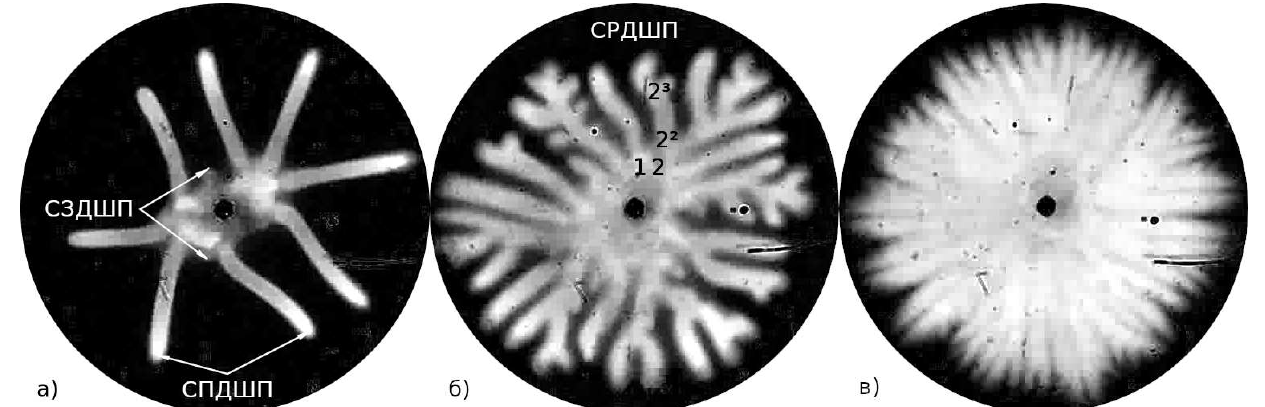
\includegraphics[width=\linewidth]{morphotypes}
            \caption{Три характерных морфотипа следов ультрабедного водородо-воздушного
                пламени в горизонтальной цилиндрической ячейке Хеле--Шоу:
                \textit{а)}~лучеобразные \textit{(6,8\,об.\,\% водорода)};
                \textit{б)}~дендритные \textit{(7,2\,об.\,\%)};
                \textit{в)}~квазиоднородные \textit{(9,0\,об.\,\%)}.
                Источник: \cite{moskalev2023}}
            \label{fig:morphotypes}
        \end{figure}

        Поэтому авторы характеризуют динамику не решением уравнения, а набором
        аппроксимирующих соотношений, оцениваемых по экспериментальным данным методом
        наименьших квадратов: фрактальной размерностью следа $d_B(x)$
        \textit{(метод клеточного покрытия)}, аппроксимированной логистической моделью;
        степенной и экспоненциальной моделями длины пути фронта $s(t)$; и
        логарифмически-экспоненциальной моделью зависимости начальной скорости фронта
        $v_0$ от объёмной концентрации водорода $x$ \textit{(рис.~\ref{fig:velocity})}.
        Эти скейлинговые соотношения играют роль эффективного <<решения>> задачи там,
        где уравнение не поддаётся прямому интегрированию.

        \begin{figure}[H]
            \centering
            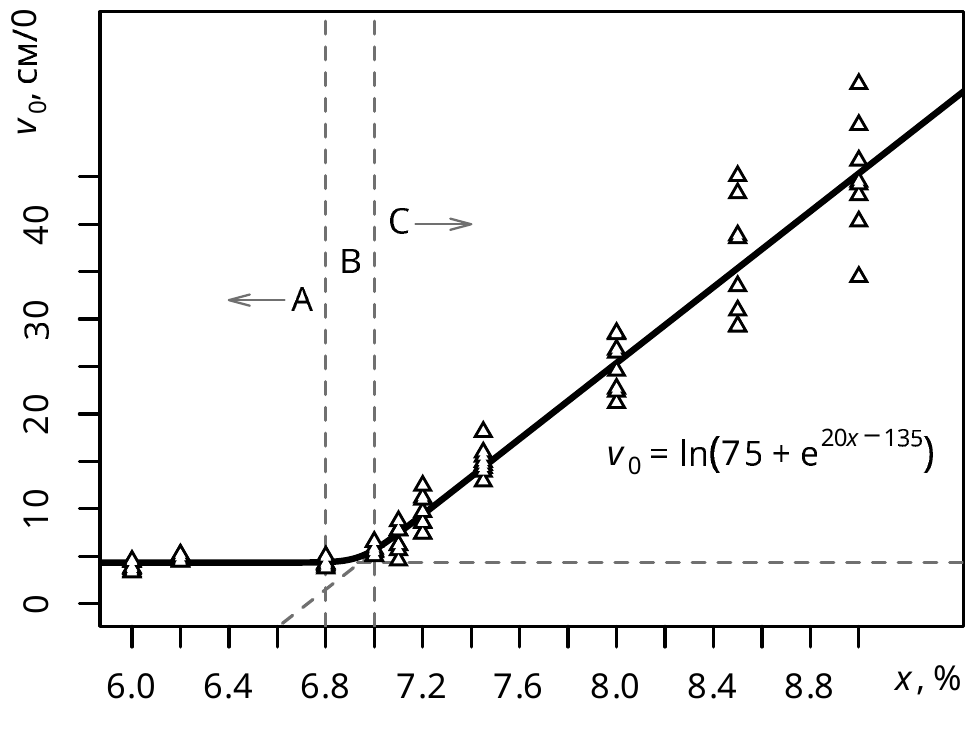
\includegraphics[width=0.68\linewidth]{velocity_v0}
            \caption{Зависимость начальной скорости фронта $v_0$ ультрабедного
                водородо-воздушного пламени от объёмной концентрации водорода $x$
                и её логарифмически-экспоненциальная аппроксимация. Источник:
                \cite{moskalev2023}}
            \label{fig:velocity}
        \end{figure}

        Таким образом, спектр методов простирается от точных аналитических решений
        \textit{(узкий класс идеализированных задач)} через универсальные численные схемы
        к феноменологическому описанию, применяемому в наиболее сложных режимах. Выбор
        метода определяется параметрами задачи \textit{($\mathrm{Pe}$, $\mathrm{Da}$)},
        геометрией области и требуемой точностью. В следующем разделе один из подходов
        доводится до конкретного примера расчёта с приведением кода.

    \unnsection{Пример расчёта}

    В предыдущем разделе было показано, что для линейного реакционного члена
    $R(c) = -kc$ и постоянных коэффициентов точное решение уравнения
    конвекции--реакции--диффузии доступно аналитически.
    Настоящий раздел конкретизирует эту идею: формулируется задача с явно
    заданными числовыми параметрами, для неё последовательными заменами переменных
    выводится точное решение, затем численно реализуется схема Кранка--Николсон
    и проводится сравнение результатов.

    \unnsubsection{Постановка конкретной задачи}

        Рассматривается одномерное уравнение конвекции--реакции--диффузии:
        \[
            \frac{\partial c}{\partial t}
            + v\,\frac{\partial c}{\partial x}
            = D\,\frac{\partial^2 c}{\partial x^2} - k c,
            \qquad x \in \mathbb{R},\quad t > 0,
        \]
        с начальным условием в виде гауссова пика, сосредоточённого в точке $x = 0$:
        \[
            c(x, 0) = \exp\!\left(-x^2\right).
        \]
        Физически задача описывает следующую ситуацию: в начальный момент времени
        в среде, движущейся с постоянной скоростью $v$, образовалось облако примеси
        с гауссовым профилем концентрации.
        При $t > 0$ облако одновременно переносится потоком (конвекция),
        расплывается за счёт молекулярного перемешивания (диффузия)
        и постепенно убывает вследствие необратимого распада примеси по реакции первого
        порядка (например, радиоактивный распад или нейтрализация загрязнителя).
        Значения параметров задачи:
        \[
            v = 0{,}5 \ \text{м/с}, \quad
            D = 0{,}1 \ \text{м}^2\!/\text{с}, \quad
            k = 0{,}2 \ \text{с}^{-1}.
        \]
        При характерном пространственном масштабе задачи $L \sim 1$\,м глобальное
        число Пекле $\mathrm{Pe} = vL/D = 5$: конвекция заметно доминирует над
        диффузией, однако оба механизма вносят ощутимый вклад.

    \unnsubsection{Аналитическое решение}

        Точная формула получается двумя последовательными заменами переменных,
        каждая из которых устраняет один из двух «возмущающих» членов.

        \textbf{Шаг~1. Устранение реакционного слагаемого.}
        Полагаем $c(x, t) = e^{-kt}\,w(x, t)$.
        Вычислим производные и подставим в уравнение:
        \[
            e^{-kt}\!\left(\frac{\partial w}{\partial t}
            + v\,\frac{\partial w}{\partial x}\right)
            = D\,e^{-kt}\frac{\partial^2 w}{\partial x^2}.
        \]
        Сокращая на $e^{-kt} > 0$, получаем уравнение конвекции--диффузии
        без реакции:
        \[
            \frac{\partial w}{\partial t}
            + v\,\frac{\partial w}{\partial x}
            = D\,\frac{\partial^2 w}{\partial x^2}, \qquad
            w(x, 0) = e^{-x^2}.
        \]

        \textbf{Шаг~2. Устранение конвективного слагаемого.}
        Переходим в систему координат, движущуюся со скоростью $v$:
        $\xi = x - vt$, $\tau = t$.
        В новых переменных полная производная по времени при постоянном $\xi$
        равна $\partial w/\partial \tau = \partial w / \partial t + v\,\partial w / \partial x$,
        поэтому уравнение конвекции--диффузии принимает вид чистого уравнения теплопроводности:
        \[
            \frac{\partial w}{\partial \tau}
            = D\,\frac{\partial^2 w}{\partial \xi^2}, \qquad
            w(\xi, 0) = e^{-\xi^2}.
        \]
        Его решение задаётся свёрткой начального условия с фундаментальным решением:
        \[
            w(\xi, \tau)
            = \int_{-\infty}^{+\infty}
              \frac{1}{\sqrt{4\pi D\tau}}\,
              e^{-(\xi-\eta)^2/(4D\tau)}\cdot
              e^{-\eta^2}\,d\eta.
        \]
        Вычислим этот интеграл, выделив полный квадрат в показателе степени:
        \begin{align*}
            -\frac{(\xi-\eta)^2}{4D\tau} - \eta^2
            &= -\frac{1+4D\tau}{4D\tau}
              \left(\eta - \frac{\xi}{1+4D\tau}\right)^{\!2}
              - \frac{\xi^2}{1+4D\tau}.
        \end{align*}
        Интеграл от гауссовой экспоненты по $\eta$ вычисляется стандартно:
        $\int_{-\infty}^{+\infty} e^{-A(\eta - B)^2}\,d\eta = \sqrt{\pi/A}$,
        откуда
        \[
            w(\xi, \tau)
            = \frac{1}{\sqrt{1+4D\tau}}\,
              \exp\!\left(-\frac{\xi^2}{1+4D\tau}\right).
        \]
        Возвращаясь к исходным переменным ($\xi = x - vt$, $\tau = t$) и
        подставляя множитель $e^{-kt}$, приходим к \textit{точному решению
        исходной задачи}:
        \[
            \boxed{
                c(x, t)
                = \frac{e^{-kt}}{\sqrt{1+4Dt}}\,
                  \exp\!\!\left(-\frac{(x - vt)^2}{1+4Dt}\right).
            }
        \]
        Формула явно разделяет вклады трёх физических механизмов.
        \textit{Конвекция} смещает центр пика со скоростью $v$: в показателе
        степени стоит $(x - vt)$, а не $x$.
        \textit{Диффузия} расширяет пик (знаменатель $1 + 4Dt$ монотонно растёт)
        и снижает его высоту (предэкспоненциальный множитель $1/\sqrt{1+4Dt}$
        убывает обратно пропорционально ширине).
        \textit{Реакция} равномерно подавляет всё поле концентрации на $e^{-kt}$,
        не меняя форму профиля.

        В таблице~\ref{tab:cmax} приведены аналитические значения максимальной
        концентрации (достигается в центре пика $x = vt$) в контрольные моменты
        времени, а также раздельный вклад диффузии и реакции.

        \begin{table}[H]
            \centering
            \label{tab:cmax}
            \begin{tabular}{lrrrrr}
                \toprule
                & $t = 0$ & $t = 1$ & $t = 2$ & $t = 3$ & $t = 5$ \\
                \midrule
                Только диффузия ($k=0$): $1/\sqrt{1+4Dt}$
                    & 1{,}000 & 0{,}845 & 0{,}745 & 0{,}674 & 0{,}577 \\
                Только реакция ($D=0$): $e^{-kt}$
                    & 1{,}000 & 0{,}819 & 0{,}670 & 0{,}549 & 0{,}368 \\
                Оба механизма: $e^{-kt}/\sqrt{1+4Dt}$
                    & 1{,}000 & 0{,}692 & 0{,}499 & 0{,}370 & 0{,}212 \\
                \bottomrule
            \end{tabular}
            \caption{Максимальная концентрация и вклад отдельных механизмов}
        \end{table}

        Из таблицы видно, что совместное действие диффузии и реакции приводит
        к значительно более быстрому убыванию максимума, чем каждый механизм
        по отдельности: к моменту $t = 5$\,с максимальная концентрация составляет
        лишь $21{,}2\,\%$ от начальной.

    \unnsubsection{Численный метод}

        Для верификации аналитического решения задача решается численно.
        Бесконечная прямая заменяется конечным отрезком $[x_l, x_r] = [-2, 10]$\,м
        с однородными граничными условиями Дирихле $c(x_l, t) = c(x_r, t) = 0$.
        Границы выбраны достаточно удалёнными: на всём промежутке $t \in [0, 5]$\,с
        точное решение в точках $x = -2$ и $x = 10$ не превышает $3\cdot10^{-4}$,
        поэтому замена бесконечной области конечной практически не влияет на решение.

        Введём равномерные сетки: $x_i = x_l + i\,\Delta x$
        ($i = 0, \ldots, N$,\ $\Delta x = 12/N$)
        и $t^n = n\,\Delta t$ ($n = 0, \ldots, M$,\ $\Delta t = T/M$).
        Схема Кранка--Николсон усредняет пространственный оператор между
        временными слоями $n$ и $n+1$:
        \[
            \frac{c_i^{n+1} - c_i^n}{\Delta t}
            = \frac{1}{2}\left[\mathcal{L}(c^n)_i
                              + \mathcal{L}(c^{n+1})_i\right],
        \]
        где пространственный оператор аппроксимируется центральными разностями:
        \[
            \mathcal{L}(c)_i
            = D\,\frac{c_{i+1} - 2c_i + c_{i-1}}{\Delta x^2}
            - v\,\frac{c_{i+1} - c_{i-1}}{2\,\Delta x}
            - k\,c_i.
        \]
        Применение центральных разностей для конвективного члена оправдано
        малостью ячеечного числа Пекле:
        \[
            \mathrm{Pe}_h
            = \frac{v\,\Delta x}{D}
            = \frac{0{,}5 \cdot 0{,}02}{0{,}1}
            = 0{,}1 \ll 2.
        \]
        Введём безразмерные коэффициенты:
        \[
            \alpha = \frac{D\,\Delta t}{2\,\Delta x^2}, \qquad
            \beta  = \frac{v\,\Delta t}{4\,\Delta x},   \qquad
            \gamma = \frac{k\,\Delta t}{2}.
        \]
        Перенося неявную часть в левую сторону, на каждом временном шаге
        необходимо решить \textit{трёхдиагональную} систему
        $A\,\mathbf{c}^{n+1} = B\,\mathbf{c}^n$
        для вектора значений во внутренних узлах.
        Матрицы $A$ (неявная) и $B$ (явная) имеют структуру:
        \[
            A:\;
            \begin{cases}
                \text{поддиагональ:} & -(\alpha+\beta), \\
                \text{главная:}      & \phantom{-}1 + 2\alpha + \gamma, \\
                \text{наддиагональ:} & -(\alpha-\beta);
            \end{cases}
            \qquad
            B:\;
            \begin{cases}
                \text{поддиагональ:} & \alpha+\beta, \\
                \text{главная:}      & 1 - 2\alpha - \gamma, \\
                \text{наддиагональ:} & \alpha-\beta.
            \end{cases}
        \]
        Схема Кранка--Николсон является \textit{безусловно устойчивой} (для
        диффузии--реакции) и имеет \textit{второй порядок точности} по времени
        и по пространству: $O(\Delta t^2 + \Delta x^2)$.
        Трёхдиагональная система решается алгоритмом прогонки,
        реализованным в функции \texttt{scipy.linalg.solve\_banded}.

    \unnsubsection{Реализация на Python}

        Ниже приведена полная программа.
        Она вычисляет аналитическое решение по явной формуле,
        параллельно проводит численную интеграцию схемой Кранка--Николсон,
        строит два графика и выводит таблицу погрешностей.
        Программу следует запустить до компиляции \LaTeX{}, чтобы
        сгенерировать файл \texttt{figures/crd\_solution.png}.

\begin{minted}{python}
import numpy as np
import matplotlib.pyplot as plt
from scipy.linalg import solve_banded

# Параметры задачи
v = 0.5 # скорость конвекции, м/с
D = 0.1 # коэффициент диффузии, м²/с
k = 0.2 # константа скорости реакции первого порядка, 1/с

x_left  = -2.0 # левая граница области, м
x_right = 10.0 # правая граница области, м
T       = 5.0  # конечный момент времени, с

# Параметры сетки
N  = 600                    # число пространственных интервалов
M  = 2000                   # число временных шагов
dx = (x_right - x_left) / N # шаг по пространству: 0.02 м
dt = T / M                  # шаг по времени: 0.0025 с

# Массивы узлов
x = np.linspace(x_left, x_right, N + 1)

# Начальное условие
c = np.exp(-x**2)

# Аналитическое решение
def c_exact(x, t):
    if t == 0.0:
        return np.exp(-x**2)
    denom = 1.0 + 4.0 * D * t
    return np.exp(-k * t) / np.sqrt(denom) * np.exp(-(x - v * t)**2 / denom)

# Коэффициенты схемы Кранка–Николсон
alpha = D * dt / (2.0 * dx**2) # диффузионный параметр
beta  = v * dt / (4.0 * dx)    # конвективный параметр
gamma = k * dt / 2.0           # реакционный параметр

# Матрица A
#   ab[0, j] = элемент наддиагонали  A[j-1, j] = -(alpha - beta)
#   ab[1, j] = диагональный элемент  A[j, j]   = 1 + 2*alpha + gamma
#   ab[2, j] = элемент поддиагонали  A[j+1, j] = -(alpha + beta)
n_inner = N - 1                   # число внутренних узлов
ab = np.zeros((3, n_inner))
ab[0, 1:]  = -(alpha - beta)      # наддиагональ
ab[1, :]   =  1 + 2*alpha + gamma # главная диагональ
ab[2, :-1] = -(alpha + beta)      # поддиагональ

# Временная интеграция
plot_times = [0.0, 1.0, 2.0, 3.0, 5.0] # моменты для записи профилей
snapshots  = {}   # словарь: t -> (c_численное, c_аналитическое)

def record(t_val, c_num):
    snapshots[t_val] = (c_num.copy(), c_exact(x, t_val))

record(0.0, c)

for n in range(M):
    ci = c[1:-1]   # значения во внутренних узлах на слое n

    # Правая часть системы: вектор B * c^n
    # B: поддиагональ = (alpha+beta),
    #    главная      = (1 - 2*alpha - gamma),
    #    наддиагональ = (alpha - beta)
    rhs = np.zeros(n_inner)

    # Первый внутренний узел:
    rhs[0] = ((1 - 2*alpha - gamma) * ci[0]
              + (alpha - beta) * ci[1])

    # Внутренние узлы:
    rhs[1:-1] = ((alpha + beta) * ci[:-2]
                 + (1 - 2*alpha - gamma) * ci[1:-1]
                 + (alpha - beta) * ci[2:])

    # Последний внутренний узел:
    rhs[-1] = ((alpha + beta) * ci[-2]
               + (1 - 2*alpha - gamma) * ci[-1])

    # Решение системы
    c_new_inner = solve_banded((1, 1), ab, rhs)

    # Сборка полного вектора с граничными условиями c = 0
    c_new = np.zeros(N + 1)
    c_new[1:-1] = c_new_inner
    c = c_new

    # Запись среза при достижении контрольного момента
    t_cur = (n + 1) * dt
    for pt in plot_times:
        if pt not in snapshots and abs(t_cur - pt) < dt / 2:
            record(pt, c)

# Визуализация результатов
fig, axes = plt.subplots(1, 2, figsize=(14, 5))
fig.suptitle("Решение уравнения конвекции–реакции–диффузии", fontsize=13)

# Левый график: профили концентрации в разные моменты времени
ax = axes[0]
colors = plt.cm.plasma(np.linspace(0.1, 0.85, len(plot_times)))
for i, pt in enumerate(plot_times):
    c_num, c_an = snapshots[pt]
    ax.plot(x, c_an,  color=colors[i], lw=2.0,
            label=f"t = {pt} с (аналит.)")
    ax.plot(x, c_num, color=colors[i], lw=1.5, ls="--",
            label=f"t = {pt} с (числен.)")
ax.set_xlabel("x, м")
ax.set_ylabel("c(x, t)")
ax.set_title("Профили концентрации примеси")
ax.legend(fontsize=7.5, ncol=2)
ax.set_xlim(x_left, x_right)
ax.set_ylim(-0.05, 1.1)
ax.grid(True, alpha=0.3)

# Правый график: убывание максимальной концентрации
ax2 = axes[1]
t_arr = np.linspace(0.0, T, 500)
c_max_both = np.exp(-k * t_arr) / np.sqrt(1.0 + 4.0 * D * t_arr)
c_max_diff = 1.0 / np.sqrt(1.0 + 4.0 * D * t_arr) # только диффузия (k=0)
c_max_rxn  = np.exp(-k * t_arr)                   # только реакция (D=0)
ax2.plot(t_arr, c_max_both, "k-",  lw=2.0,
         label="Оба эффекта (диффузия + реакция)")
ax2.plot(t_arr, c_max_diff, "b--", lw=1.5,
         label="Только диффузия ($k=0$)")
ax2.plot(t_arr, c_max_rxn,  "r:",  lw=1.5,
         label="Только реакция ($D=0$)")
ax2.set_xlabel("t, с")
ax2.set_ylabel("max c(x, t)")
ax2.set_title("Убывание максимальной концентрации")
ax2.legend()
ax2.grid(True, alpha=0.3)

plt.tight_layout()
plt.savefig("figures/crd_solution.png", dpi=150, bbox_inches="tight")
plt.show()

# Таблица максимальных абсолютных погрешностей
print(f"\n{"t, с":>6} | {"max |c_числ - c_аналит|":>25}")
print("-" * 35)
for pt in plot_times[1:]:
    c_num, c_an = snapshots[pt]
    err = np.max(np.abs(c_num - c_an))
    print(f"{pt:>6.1f} | {err:>25.2e}")
\end{minted}

    \unnsubsection{Результаты и их анализ}

        После запуска программы в консоли выводится таблица максимальных
        абсолютных погрешностей, а в файл сохраняются два графика
        (рис.~\ref{fig:crd_solution}).

\begin{minted}[linenos=false]{text}
  t, с |   max |c_числ - c_аналит|
-----------------------------------
   1.0 |                  8.66e-03
   2.0 |                  5.40e-03
   3.0 |                  3.72e-03
   5.0 |                  1.98e-03
\end{minted}

        \begin{figure}[H]
            \centering
            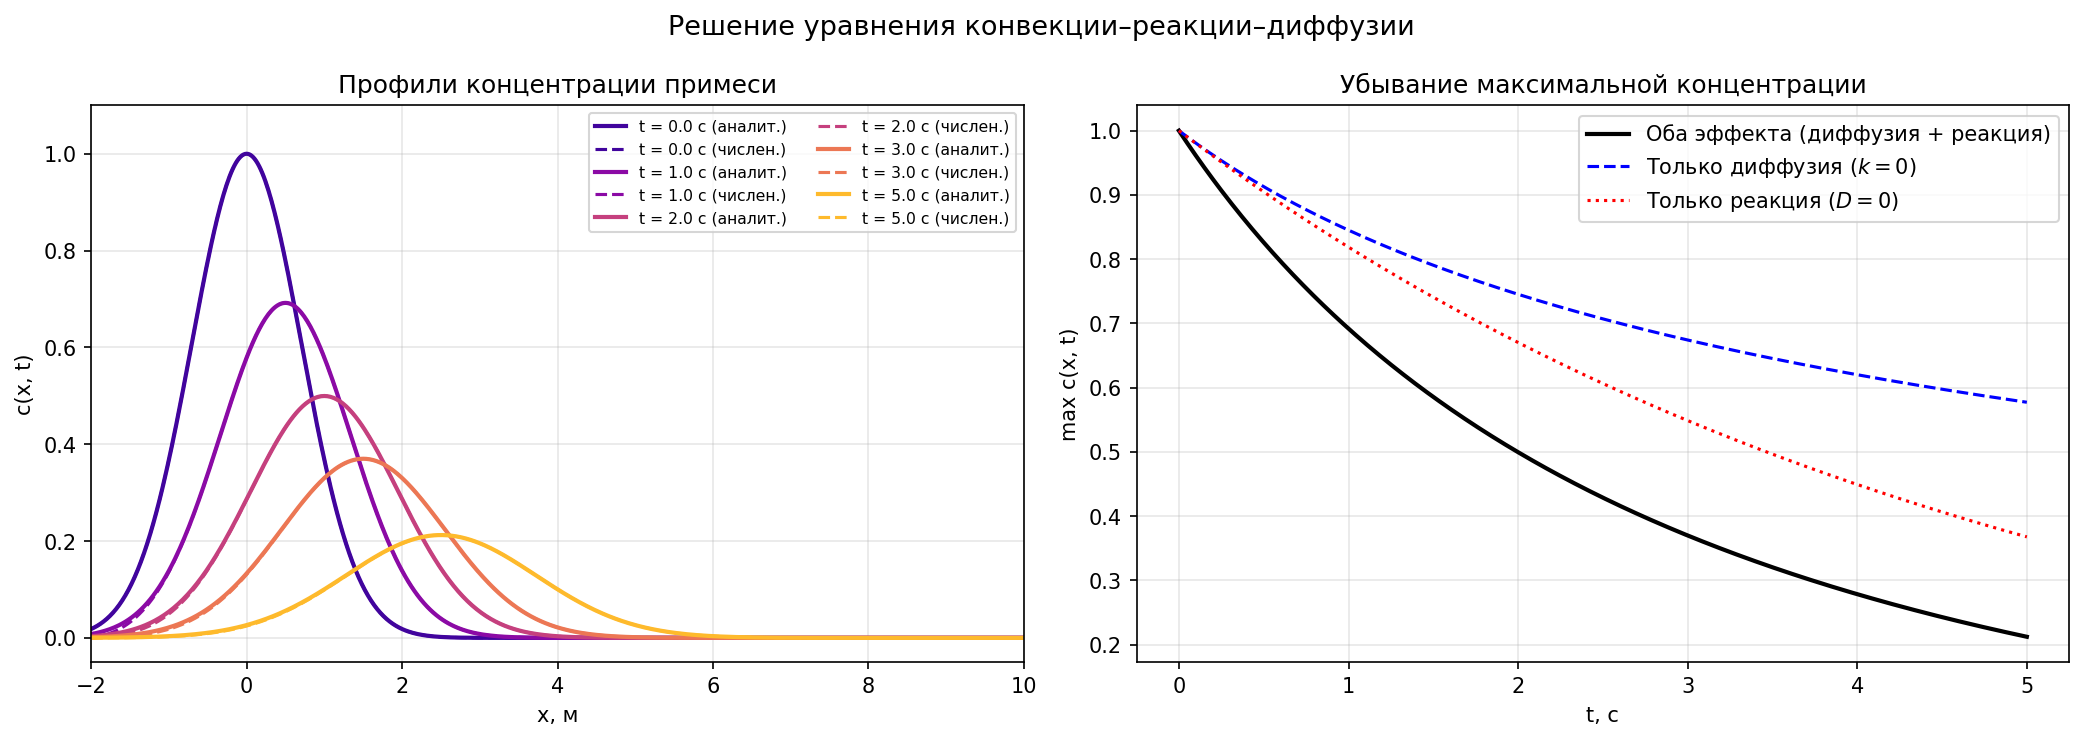
\includegraphics[width=\linewidth]{crd_solution}
            \caption{Слева: профили концентрации $c(x,t)$ в моменты $t = 0, 1, 2, 3, 5$\,с;
                     сплошные линии~--- аналитическое решение,
                     штриховые~--- схема Кранка--Николсон.
                     Справа: убывание максимальной концентрации с разбивкой
                     на вклад диффузии и реакции.}
            \label{fig:crd_solution}
        \end{figure}

        \textbf{Левый график} показывает эволюцию профиля концентрации.
        Центр гауссова пика движется вправо со скоростью $v = 0{,}5$\,м/с
        (за 5\,с смещается на 2{,}5\,м), пик постепенно уширяется и
        одновременно убывает по амплитуде.
        Штриховые (численные) кривые практически сливаются со сплошными
        (аналитическими), что свидетельствует о высокой точности схемы.

        \textbf{Правый график} наглядно демонстрирует, что суммарное убывание
        максимума (чёрная кривая) происходит значительно быстрее, чем
        от каждого механизма в отдельности:
        к моменту $t = 5$\,с только диффузия снизила бы максимум до
        $57{,}7\,\%$ от начального значения, только реакция~--- до $36{,}8\,\%$,
        а оба эффекта вместе~--- до $21{,}2\,\%$.
        Это объясняется тем, что в аналитической формуле диффузионный множитель
        $1/\sqrt{1+4Dt}$ и реакционный $e^{-kt}$ входят \textit{произведением},
        а не суммой: их совместное действие мультипликативно.

        \textbf{Таблица погрешностей}, выводимая программой в консоль,
        показывает, что максимальное отклонение численного решения от
        аналитического не превышает $10^{-2}$ и монотонно убывает со временем.
        Доминирующий источник погрешности~--- не усечение разностной схемы,
        а несоответствие граничных условий: аналитическое решение получено для
        бесконечной прямой, тогда как численно задача решается на отрезке $[-2, 10]$\,м
        с условием $c = 0$ на краях.
        В начальный момент это условие нарушено на величину
        $c(-2, 0) = e^{-4} \approx 0{,}018$; именно этим объясняется
        начальная погрешность порядка $10^{-2}$.
        По мере того как плюм смещается вправо, концентрация у левой границы
        экспоненциально убывает, что и приводит к уменьшению погрешности
        с ростом $t$.


    % Список литературы (управляется флагом \ifbib в config.tex)
    \ifbib
        % Страница со списком литературы
\cleardoublepage

% Переключаем стиль на empty: нет шапки и нет номера страницы
\pagestyle{empty}

% Делаем так, чтобы библиография появлялась независимо от ссылок
\nocite{*}

% Компактная верстка библиографии
\renewcommand{\bibfont}{\small}
\setlength{\bibitemsep}{2pt plus 1pt minus 1pt}
\setlength{\bibparsep}{0pt}
\setlength{\bibhang}{1.5em}

% Выводим библиографию по центру
\begin{center}
    \printbibliography[heading=bibintoc, title={Список литературы}]
\end{center}

    \fi

% Конец документа
\end{document}
